%%%%%%%%%%%%%%%%%%%%%%%%%%%%%%%%%%%%%%%%%%%%%%%%%%%%%%%%%%%%%%%%%%
%%%%%%%%%%%%%%%%%%%%%%%%%%%%%%%%%%%%%%%%%%%%%%%%%%%%%%%%%%%%%%%%%%
%Packages
\documentclass[10pt, a4paper]{article}
\usepackage[top=3cm, bottom=4cm, left=1.5cm, right=1.5cm]{geometry}
\usepackage{amsmath,amsthm,amsfonts,amssymb,amscd, fancyhdr, color, comment, graphicx, environ}
\usepackage{float}
\usepackage{mathrsfs}
\usepackage[math-style=ISO]{unicode-math}
\setmathfont{TeX Gyre Termes Math}
\usepackage{lastpage}
\usepackage[dvipsnames]{xcolor}
\usepackage[framemethod=TikZ]{mdframed}
\usepackage{enumerate}
\usepackage[shortlabels]{enumitem}
\usepackage{fancyhdr}
\usepackage{indentfirst}
\usepackage{listings}
\usepackage{sectsty}
\usepackage{thmtools}
\usepackage{shadethm}
\usepackage{hyperref}
\usepackage{setspace}
\hypersetup{
    colorlinks=true,
    linkcolor=blue,
    filecolor=magenta,      
    urlcolor=blue,
}
\usepackage{tcolorbox}
\tcbuselibrary{skins,xparse}

\usepackage{wrapfig}

%%%%%%%%%%%%%%%%%%%%%%%%%%%%%%%%%%%%%%%%%%%%%%%%%%%%%%%%%%%%%%%%%%
%%%%%%%%%%%%%%%%%%%%%%%%%%%%%%%%%%%%%%%%%%%%%%%%%%%%%%%%%%%%%%%%%%
%Environment setup
\mdfsetup{skipabove=\topskip,skipbelow=\topskip}
\newrobustcmd\ExampleText{%
An \textit{inhomogeneous linear} differential equation has the form
\begin{align}
L[v ] = f,
\end{align}
where $L$ is a linear differential operator, $v$ is the dependent
variable, and $f$ is a given non−zero function of the independent
variables alone.
}
\mdfdefinestyle{theoremstyle}{%
linecolor=black,linewidth=1pt,%
frametitlerule=true,%
frametitlebackgroundcolor=gray!0,
innertopmargin=\topskip,
}
\mdtheorem[style=theoremstyle]{Problem}{Problem}
\newenvironment{Solution}{\textbf{Solution.}}

\definecolor{codegreen}{rgb}{0,0.6,0}
\definecolor{codegray}{rgb}{0.5,0.5,0.5}
\definecolor{codepurple}{rgb}{0.58,0,0.82}
\definecolor{backcolour}{rgb}{0.95,0.95,0.92}

\lstdefinestyle{mystyle}{
    backgroundcolor=\color{backcolour},   
    commentstyle=\color{codegreen},
    keywordstyle=\color{magenta},
    numberstyle=\tiny\color{codegray},
    stringstyle=\color{codepurple},
    basicstyle=\ttfamily\footnotesize,
    breakatwhitespace=false,         
    breaklines=true,                 
    captionpos=b,                    
    keepspaces=true,                 
    numbers=left,                    
    numbersep=5pt,                  
    showspaces=false,                
    showstringspaces=false,
    showtabs=false,                  
    tabsize=2
}

\lstset{style=mystyle}
%%%%%%%%%%%%%%%%%%%%%%%%%%%%%%%%%%%%%%%%%%%%%%%%%%%%%%%%%%%%%%%%%%
%%%%%%%%%%%%%%%%%%%%%%%%%%%%%%%%%%%%%%%%%%%%%%%%%%%%%%%%%%%%%%%%%%
%Fill in the appropriate information below
\newcommand{\norm}[1]{\left\lVert#1\right\rVert}     
\newcommand\course{XXXX0000}                            % <-- course name   
\newcommand\hwnumber{0}                                 % <-- homework number
\newcommand\Information{Someone}                        % <-- personal information
%%%%%%%%%%%%%%%%%%%%%%%%%%%%%%%%%%%%%%%%%%%%%%%%%%%%%%%%%%%%%%%%%%
%%%%%%%%%%%%%%%%%%%%%%%%%%%%%%%%%%%%%%%%%%%%%%%%%%%%%%%%%%%%%%%%%%
%Page setup
\pagestyle{fancy}
\headheight 35pt
\lhead{sept-dec 2023}
\rhead{
\includegraphics[width=2.5cm]{logo.png}}
\lfoot{}
\pagenumbering{arabic}
\cfoot{\small\thepage}
\rfoot{}
\headsep 1.2em
\renewcommand{\baselinestretch}{1.25}
%%%%%%%%%%%%%%%%%%%%%%%%%%%%%%%%%%%%%%%%%%%%%%%%%%%%%%%%%%%%%%%%%%
%%%%%%%%%%%%%%%%%%%%%%%%%%%%%%%%%%%%%%%%%%%%%%%%%%%%%%%%%%%%%%%%%%
%Add new commands here
\renewcommand{\labelenumi}{\alph{enumi})}
\newcommand{\Z}{\mathbb Z}
\newcommand{\R}{\mathbb R}
\newcommand{\Q}{\mathbb Q}
\newcommand{\NN}{\mathbb N}
\newcommand{\PP}{\mathbb P}
\DeclareMathOperator{\Mod}{Mod} 
\renewcommand\lstlistingname{Algorithm}
\renewcommand\lstlistlistingname{Algorithms}
\def\lstlistingautorefname{Alg.}
\newtheorem*{theorem}{Theorem}
\newtheorem*{lemma}{Lemma}
\newtheorem{case}{Case}
\newcommand{\assign}{:=}
\newcommand{\infixiff}{\text{ iff }}
\newcommand{\nobracket}{}
\newcommand{\backassign}{=:}
\newcommand{\tmmathbf}[1]{\ensuremath{\boldsymbol{#1}}}
\newcommand{\tmop}[1]{\ensuremath{\operatorname{#1}}}
\newcommand{\tmtextbf}[1]{\text{{\bfseries{#1}}}}
\newcommand{\tmtextit}[1]{\text{{\itshape{#1}}}}

\newenvironment{itemizedot}{\begin{itemize} \renewcommand{\labelitemi}{$\bullet$}\renewcommand{\labelitemii}{$\bullet$}\renewcommand{\labelitemiii}{$\bullet$}\renewcommand{\labelitemiv}{$\bullet$}}{\end{itemize}}
\catcode`\<=\active \def<{
\fontencoding{T1}\selectfont\symbol{60}\fontencoding{\encodingdefault}}
\catcode`\>=\active \def>{
\fontencoding{T1}\selectfont\symbol{62}\fontencoding{\encodingdefault}}
\catcode`\<=\active \def<{
\fontencoding{T1}\selectfont\symbol{60}\fontencoding{\encodingdefault}}

%%%%%%%%%%%%%%%%%%%%%%%%%%%%%%%%%%%%%%%%%%%%%%%%%%%%%%%%%%%%%%%%%%
%%%%%%%%%%%%%%%%%%%%%%%%%%%%%%%%%%%%%%%%%%%%%%%%%%%%%%%%%%%%%%%%%%
%Begin now!



\begin{document}

\begin{titlepage}
    \begin{center}
            
        \huge
        \textbf{SAÉ 1.01 - Reporting à partir de données stockées dans un SGBD relationnel }
            
        \LARGE
        \textit{Fascicule de travail : naissance de reporting }
            
        \vspace{1cm}
            \small
        \begin{tabular}{|c|l|}\hline
             Compétence ciblée&  Traiter les données à des fins décisionnelles   \\\
             & Niveau 1 : Traiter des données structurées   \\\hline
             AC couverts& Correctement interpréter et prendre en compte le besoin du commanditaire ou du client   \\
             &  Respecter les formalismes de notation   \\
             &  Connaître la syntaxe des langages et savoir l’utiliser   \\
             & Mesurer l’importance de maîtriser la structure des données à exploiter   \\ \hline
              & La mise à jour et la présentation des tableaux de bord sont essentielles au suivi de   l’activité  d’une \\
             Objectifs de la & entreprise. En tant que chargé d’analyse et de reporting, l’étudiant pourra être amené à produire \\
             SAÉ  et  &  de tels tableaux de bord en support aux services de pilotage de l’activité.\\
                problématique & Il devra pour cela assurer la sélection et l’export des données utiles, notamment celles stockées dans\\
              professionnelle &  des bases de données, les analyser et les restituer avec les outils adaptés.\\
                & Les objectifs de cette SAÉ sont les suivants : \\
                & – Amener l’étudiant à construire des indicateurs de performance ainsi que les restituer sous forme\\
                &  de tableau de bord\\
                & – Identifier les besoins clients et être force de proposition pour s’adapter à ces besoins.\\
                & – Se confronter à des difficultés dans les bases de données rencontrées\\ \hline
                & L’étudiant est mis en situation de production de tableaux de bord à partir de données stockées \\
               Description & dans un SGBD relationnel, en respectant les termes d’un cahier des charges fourni (spécification,\\
                & livrables, délai... ). La base de données fournie présente un certain nombre de difficultés que l’on \\
                & peut rencontrer dans une situation professionnelle réelle (BD plus grande, jointures complexes, ....).\\
                & Le cahier des charges présente le schéma relationnel de la BD à utiliser, les demandes de tableaux de \\
                & bords et reporting. L’étudiant doit produire l’ensemble des scripts permettant d’extraire les données \\
                &nécessaires et réaliser les livrables demandés.\\
                &Il doit en outre documenter le code et le résultat obtenu\\ \hline
                Heures formation&5hTD\\\hline
                Heures de projet tutoré&12h projet\\\hline
                Ressources mobilisées&– R1.01 | Tableur et reporting\\
                &– R1.02 | Bases de données relationnelles 1\\
                &– R1.10 | Projet Personnel et Professionnel 1\\\hline
                Type de rendu : & Rapport de réalisation + codes commentés + reporting produit\\
                Livrable  & SGBD, ACCESS\\\hline
                Semestre&Semestre 1\\\hline
        \end{tabular} 
        \vfill
        
            
            
        
\includegraphics[width=0.4\textwidth]{logo.png}
        \\
            
    \end{center}
\end{titlepage}

%%%%%%%%%%%%%%%%%%%%%%%%%%%%%%%%%%%%%%%%%%%%%%%%%%%%%%%%%%%%%%%%%%
%%%%%%%%%%%%%%%%%%%%%%%%%%%%%%%%%%%%%%%%%%%%%%%%%%%%%%%%%%%%%%%%%%
%Start the assignment now
%%%%%%%%%%%%%%%%%%%%%%%%%%%%%%%%%%%%%%%%%%%%%%%%%%%%%%%%%%%%%%%%%%
%New problem



\newpage
\normalsize
\section{Cours}
\paragraph{Introdution}
Il semble aisé de collecter des données et de calculer quelques valeurs, comme des moyennes, 
puis de les interpréter abusivement. Il est en revanche beaucoup plus complexe de le faire dans un cadre scientifique rigoureux.

 Tout citoyen, qu’il soit informaticien, biologiste, chimiste, économiste, etc., est confronté à des données et statistiques qu’il doit savoir analyser avec recul. L'analyste des données doit en plus comprendre les mécanismes sous-jacents qui apparaissent lors des rendus visuels. 

Les professionnels des données s'intéressent aux trois questions :\textit{ comment collecter les données (quelles dimensions) ? comment les analyser (que permettent les données de conclure) ? et comment les présenter ?}


Les probabilités sont un domaine des mathématiques ayant pour objet l’étude de l’incertitude et du hasard. Il
ne faut pas confondre probabilités et statistique. Un processus stochastique (probabiliste) peut servir à produire des
données que l’on peut analyser de façon statistique. De même, on cherche souvent, à partir d’un jeu de données, à
modéliser leur apparition comme si elle venait d’un processus probabiliste, afin d’en déduire des modèles théoriques
et prédicatifs. \footnote{Inspiré du cours de M. Héam}




\begin{tcolorbox}[lefttitle=2cm,colback=white, colframe=gray!75!black, title=\textbf{Analyse d'une datavisualisation issue d'un reportage de France3}]
\begin{enumerate}
    \item Quelles sont les données ?
    \item Quelle visualisation choisie (et pourquoi) ?
    \item Quelle(s) erreur(s) ?
    \item Conclusion ?
\end{enumerate}

\begin{figure}[H]
    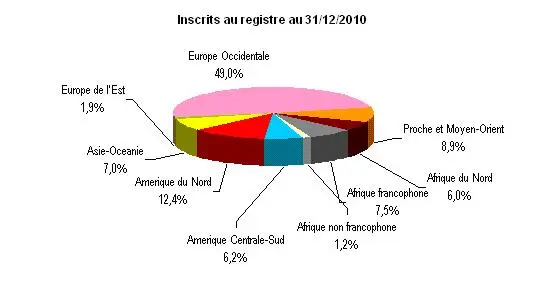
\includegraphics[scale = 0.5]{chapitre1/figures/Camembert-expat.png}
    \label{fig:France3}
\end{figure}
\vspace{3.5cm}


\end{tcolorbox}








Lorsque l’on présente des résultats statistiques pour comparer des proportions, il est fréquent d’utiliser des camemberts ou des histogrammes. Un exemple est donné dans la Figure~\ref{fig:France3} \footnote{\url{http://france3-regions.blog.francetvinfo.fr/ftv-expats/2011/12/04/qui-sont-les-nouveaux-expatries-francais.html}}. Cette présentation, en relief, est fréquemment
utilisée car plus jolie. Cependant, elle est tendancieuse, car ce que l’oeil compare les aires des différents secteurs, et l’utilisation de tranches (pour le relief) donne visuellement un poids plus fort aux données placées devant. 
Par exemple,
sur la Figure~\ref{fig:France3}, l’Europe Occidentale occupe 50\% de la surface de l’ellipse marquant le camenbert, mais bien moins
de 50\% de la surface totale du dessin, alors que cela devrait être le cas. De même, on peut remarque que l’Europe
de l’Est paraît occuper une part moins importante que l’Afrique non francophone, ce qui n’est pas le cas. De même
l’Amérique Centrale-Sud occupe plus place que le Proche et Moyen-Orient sur le dessin, alors que cela ne devrait pas
être le cas. Dans un camembert en relief, les données placées sur l’avant ont tendance à être surestimées. 

En pratique il
convient donc de ne pas utiliser les camembert en relief, ou, lorsque cela est fait, il faut choisir une très faible épaisseur
relativement au rayon du disque et une inclinaison par trop importante, afin de minimiser le biais. De même tout
découpage en tranche (en faisant ressortir une tranche) ajoute de l’épaisseur visuelle et accentue l’effet visuel. Il est
aussi important de faire attention aux couleurs : des couleurs vives, comme le rouges, attirent plus l’oeil.

\newpage

\begin{tcolorbox}[lefttitle=2cm, colframe=gray!75!black, colback=white, title=\textbf{EXERCICE 1 : Analyse de trois datavisualisations de données.}]

\begin{minipage}{0.45\textwidth}

Pour chacune de ces datavisualisation, donnez

\begin{enumerate}
    \item les éléments mis en avant, à travers les biais
    \item ce que la représentation veut montrer
    \item un titre 
\end{enumerate}
\end{minipage} \hfill
\begin{minipage}{0.7\textwidth}
\scalebox{0.8}{
    \begin{tabular}{|c|c|}\hline
       Professions intermédiaires  &  21,8390804597701\\\hline
       Agriculteurs exploitants  &  8,76436781609196\\\hline
       Cadres et professions intellectuelles supérieures  &  36,2068965517241\\\hline
       Artisans, commerçants et chefs d’entreprise  &  16,5948275862069\\\hline
       Employés et ouvriers qualifiés  &  9,98563218390805\\\hline
       Employés et ouvriers non qualifiés  &  6,60919540229885\\\hline
    \end{tabular}}
%    \caption{Catégorie socioprofessionnelle du père\footnote{source : \url{https://www.insee.fr/fr/statistiques/4797592?sommaire=4928952\#graphique-Figure3_radio1}}}	
    \label{tab:my_label}
\end{minipage}


\begin{figure}[H]
    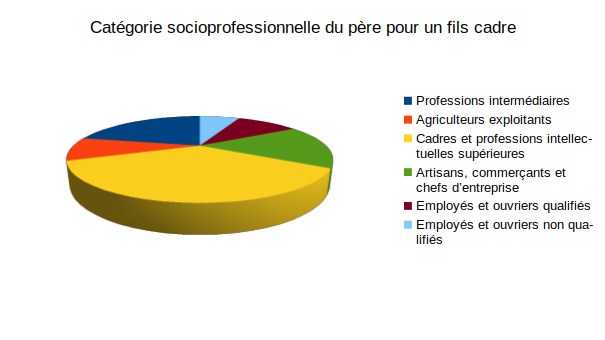
\includegraphics[scale =0.47, trim={0 3cm 0 0},clip]{chapitre1/figures/img1.png}
    \caption{}
    \label{fig:enter-label}
\end{figure}

\begin{figure}[H]
    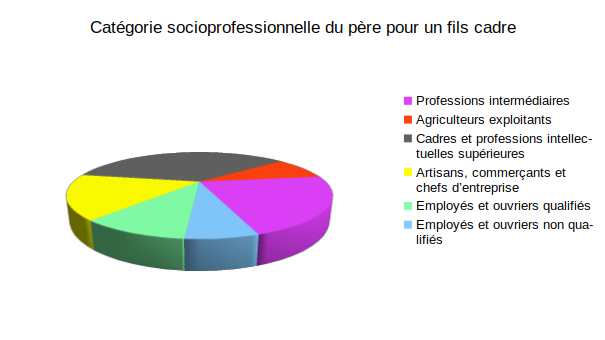
\includegraphics[scale =0.47, trim={0 2cm 0 0},clip]{chapitre1/figures/img2.png}
    \caption{}
    \label{fig:enter-label}
\end{figure}

\begin{figure}[H]
    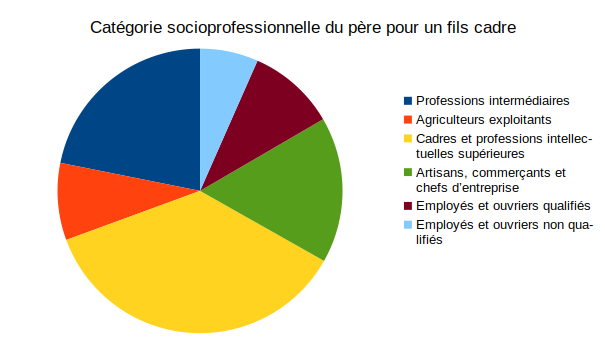
\includegraphics[scale =0.47]{chapitre1/figures/img.png}
    \caption{}
    \label{fig:enter-label}
\end{figure}

\end{tcolorbox}





\begin{tcolorbox}[lefttitle=2cm, colframe=gray!75!black, colback=white, title=\textbf{EXERCICE 2 : Analyse de trois datavisualisations de données.}]




Le problème de lien entre une valeur et l’aire représentée est aussi délicat à gérer sur les cartes. On
considère par exemple trois communes disposées comme sur la carte ci-dessous et gérée par le même commissariat.
Plus la couleur est foncée, plus le nombre de cambriolages est important. Le dessin de gauche représente la situation
en 2000 et celle de droite en 2010.

\begin{figure}[H]
    \centering
    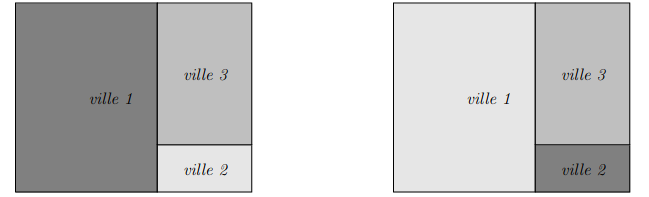
\includegraphics[scale =0.5]{chapitre1/figures/villes.png}
    \caption{Criminalité}
    \label{fig:crim1}
\end{figure}
\begin{tcolorbox}[lefttitle=2cm, colback=white, colframe=gray!95!black, title=\textbf{EXERCICE 2.1 : Analyse de la Figure~\ref{fig:crim1}}]
\begin{enumerate}
    \item Peut-on dire que la situation s’est améliorée ? 
    \item Comment faudrait il griser la carte pour que cela soit visuellement
pertinent ?
\end{enumerate}
\vspace{1.5cm}
\end{tcolorbox}

\begin{tcolorbox}[lefttitle=2cm, colback=white,colframe=gray!95!black, title=\textbf{EXERCICE 2.2 : Nouvelle analyse}]
On considère maintenant la figure ci-dessous où plus une ville est foncée, plus il y a de cambriolage par hectare de la ville, encore une fois en 2000 et 2010.

\begin{figure}[H]
    \centering
    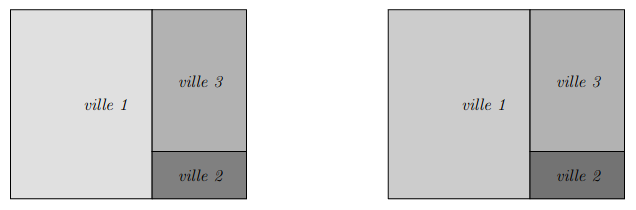
\includegraphics[scale =0.5]{chapitre1/figures/villes2.png}
    \caption{Nouvelle représentation de la criminalité}
    \label{fig:enter-label}
\end{figure}


Cela permet il de savoir où il est préférable d’habiter si l’on craint
les cambriolages ?
\vspace{2cm}

\end{tcolorbox}






\end{tcolorbox}






\begin{tcolorbox}[lefttitle=2cm, colframe=gray!75!black, colback=white, title=\textbf{EXERCICE 3 : Toujours de l'analyse de représentation}]


Pour cette représentation graphique issue de l'INSEE \footnote{Source : Insee, enquêtes Formation et qualification professionnelle (FQP) 1977, 1985, 1993, 2003 et 2014-2015.}, donnez

\begin{enumerate}
    \item le(s) biais
    \item les éléments mis en avant, à travers le(s) biais
    \item ce que la représentation veut montrer
    \item un titre 
\end{enumerate}
\begin{figure}[H]
    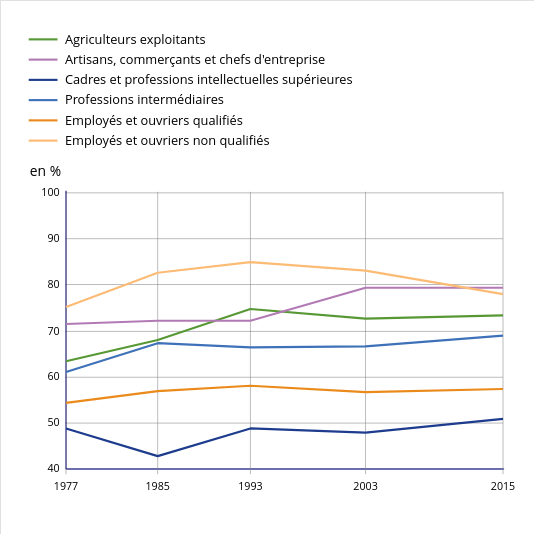
\includegraphics[scale =0.5]{chapitre1/figures/grapheF.png}
    \caption{}
    \label{fig:enter-label}
\end{figure}

\vspace{5cm}
\end{tcolorbox}

\newpage




\section{Paradoxe de Simpson}





\begin{tcolorbox}[lefttitle=2cm, colframe=gray!75!black, colback=white, title=\textbf{EXERCICE 4 : Paradoxe de Simpson}]


On considère deux lycées, notés A et B. On observe les taux de réussites suivants dans les deux lycées

\begin{minipage}{0.4\textwidth}
\textbf{Taux de réussite représentation 1}
   \centering
    
    \begin{tabular}{|c|c|c|} \hline
        &Lycée A   & Lycée B \\\hline
         garçons& 70\%& 71.05\%\\\hline
         filles &75\%& 80\%\\\hline
    \end{tabular}

\end{minipage} \hfill
\begin{minipage}{0.6\textwidth}

\begin{tcolorbox}[lefttitle=1cm, colframe=gray!75!black, colback=white, title=\textbf{EXERCICE 4.1 : représentation 1}]
\begin{enumerate}
    \item Quel lycée a le meilleur taux de réussite ?
\end{enumerate}
\vspace{1cm}

\end{tcolorbox}

\end{minipage}

\vspace{0.5cm}

\begin{tcolorbox}[lefttitle=1cm, colframe=gray!75!black, colback=white, title=\textbf{EXERCICE 4.2 : représentation 2}]
On considère maintenant les effectifs des deux lycées donnés ci-dessous. 


\begin{minipage}{0.4\textwidth}
\textbf{Effectif des lycées}
   \centering
    \begin{tabular}{|c|c|c|} \hline
        &Lycée A   & Lycée B \\\hline
         garçons &100& 100\\\hline
         filles &190& 10\\\hline
    \end{tabular}

\end{minipage} \hfill
\begin{minipage}{0.6\textwidth}


\begin{enumerate}
    \item Calculer le taux de réussite de chaque lycée. 
    \item Qu’en déduire ?
\end{enumerate}
\end{minipage}


\vspace{3cm}

\end{tcolorbox}

\end{tcolorbox}







Ce qu’il est important de retenir, c’est qu’il est facile (et malheureusement usuel) d’utiliser des représentations
graphiques trompeuses. Par ailleurs, il est parfois difficile d’obtenir les valeurs pertinentes permettant d’en tirer des
conclusions utiles. Deux exemples : 
\begin{itemize}
    \item il y a en France plus de commotion cérébrale dû à des accidents de la route sur
des piétons que sur des vélos. Certaines associations d’utilisateur de vélos l’utilise pour que le port du casque ne soit
pas rendu obligatoire. Mais ces chiffres doivent être rapportés aux volume du trafic vélo et du trafic piétons. Se pose
alors la question de choisir la mesure du trafic (en temps passé ou en kilomètres parcourus ?) et de savoir le mesurer
(actuellement on ne sait le faire qu’avec un facteur 100 près).
\item  Toujours sur la sécurité routière, il est par exemple
aussi difficile de comparer la dangerosité des routes entre deux pays comme la France et le Royaume-Uni. On peut
bien entendu compter le nombre d’accidents mortels selon des critères identiques, mais doit on rapporter ce total
au nombre de véhicule ? au nombre d’habitants ? au nombre de kilomètres parcourus ? au nombre de kilomètres de
route ? Par ailleurs, le trafic n’est pas du tout le même en France (pays de transits entre l’Europe du Nord et du Sud)
et le Royaume-Uni qui est une île. De même, on sait que les conditions météorologiques influencent sensiblement le
nombre d’accidents. Comment le prendre en compte ? 
\end{itemize}


En conclusion, il faut en statistique avoir les bonnes données
(cela demande une expertise métier en général), en nombre suffisant, et savoir restituer ces résultats convenablement.
\newpage
\section{Phénomène de Rogers}

Le phénomène de Rogers peut traduire qu’il est possible, avec de même données, de donner des résultats aux conclusion différentes. Cela montre qu’il est possible de truquer des résultat sans pour autant truquer des données,
par un moyen purement mathématique. 


\begin{tcolorbox}[lefttitle=1cm, colframe=gray!75!black, colback=white, title=\textbf{EXERCICE 5}]


Imaginons une IUT dans lequel il y a deux groupes de niveaux A et B. Les
étudiants du groupe A sont, en général, meilleur que ceux du groupe B. Une année, les groupes A a eu 14.2 de moyenne et le groupe B a eu 8 de moyenne.

La seconde année, les notes du groupe A sont : 16, 15, 15, 13, 11. 

Les notes du groupe B sont 13, 8, 6 et 3. 


\begin{tcolorbox}[lefttitle=1cm, colframe=gray!75!black, colback=white, title=\textbf{EXERCICE 5.1}]

\begin{itemize}
    \item Calculer la moyenne des groupes $A$ et $B$ 
    \item Quelle est l'évolution des moyennes sur les deux années ? 
    \item et quelle est la moyenne des deux moyennes ? 
\end{itemize}
\vspace{1cm}
\end{tcolorbox}

L’enseignant décide alors de faire passer le plus mauvais étudiant du groupe A dans le groupe B.

\begin{tcolorbox}[lefttitle=1cm, colframe=gray!75!black, colback=white, title=\textbf{EXERCICE 5.2}]


Les notes du groupe A deviennent alors 16, 15, 15 et 13.
Les notes du groupe B sont 13, 11, 8, 6 et 3. 
\begin{itemize}
    \item Calculer la moyenne des groupes $A$ et $B$ 
    \item Quelle est l'évolution des moyennes sur les deux années ?
    \item Et quelle est la moyenne des deux moyennes ?  
    \item Que déduisez-vous ?
\end{itemize}
\vspace{3cm}

\end{tcolorbox}

\end{tcolorbox}


%La moyenne du groupe A est de 14 et celle du groupe B de 7.5. Les résultats semblent donc moins bon que l’année précédente. L’enseignant décide alors de faire passer le plus mauvais étudiant du groupe A dans le groupe B.

%De cette façon, les moyennes des groupes A et B ont augmenté !
%Cela montre qu’il faut faire attention avec les moyennes, et surtout avec les moyennes de moyennes


\vspace{3cm}



\begin{tcolorbox}[lefttitle=1cm, colframe=gray!75!black, colback=white, title=\textbf{Exercice 6 : Les dés non transitifs}]
On suppose que l’on a trois dés à 6 faces, appelés A, B et C. Lors d’un lancer, pour chaque dé, chaque
face sort avec une probabilité 1/6 : les dés ne sont pas pipés.
\begin{itemize}
    \item le dé A a sur ses faces 2,2,4,4,9,9,
    \item le dé B a pour sa part 1,1,6,6,8,8,
    \item le dé C a 3,3,5,5,7,7.
\end{itemize}


\begin{tcolorbox}[lefttitle=1cm, colframe=gray!75!black, colback=white, title=\textbf{EXERCICE}]

On s’intéresse à un jeu à deux joueurs où chacun prend un dé, le lance et celui qui a le plus grand résultat gagne.

\begin{enumerate}
    \item Si j’ai le dé A et mon adversaire le B, quelle est la probabilité que je gagne ?
    \item Si j’ai le dé B et mon adversaire le C, quelle est la probabilité que je gagne ?
    \item Si j’ai le dé C et mon adversaire le A, quelle est la probabilité que je gagne ?
    \item Quel est le dé le plus fort ?
\end{enumerate}

\vspace{6cm}

\end{tcolorbox}

\end{tcolorbox}





\newpage
\section{Mise en pratique}



\begin{tcolorbox}[lefttitle=1cm, colframe=gray!75!black, colback=white, title=\textbf{ENTREE : un SGBD relationnel}]
Un SGBD relationnel.
\begin{figure}[H]
    \centering
    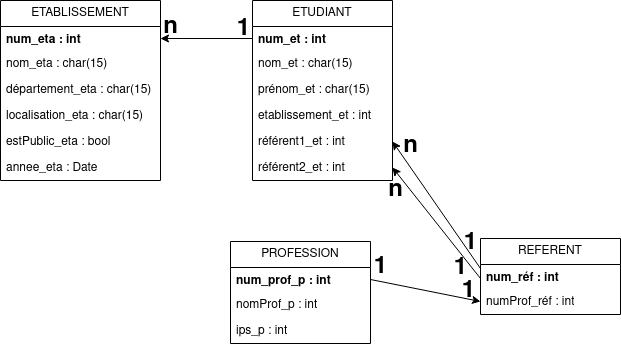
\includegraphics[scale=0.5]{chapitre1/figures/sae1UML.png}
    \caption{Diagramme UML étudié}
    \label{fig:enter-label}
\end{figure}

Un csv est disponible sous le lien suivant : lien

\end{tcolorbox}




\begin{tcolorbox}[lefttitle=1cm, colframe=gray!75!black, colback=white, title=\textbf{En sortie : A rendre. Quel modèle de gestion des
professeurs pour l’école de demain ?}]

\textbf{A rendre} : Un classeur Excel qui obtiendra les données nécessaires pour produire un certain nombre de
graphiques et tableaux.
Vous pouvez d'ors et déjà réfléchir aux données nécessaires et à la façon de concevoir les tableaux
et graphiques qui pourraient être demandés.
%Par exemple :
%\begin{itemize}
%    \item Le nombre de création d'entreprises par année et par activité
%    \item Le nombre d'entreprises présentes sur un territoire (département, région) pour une année i.
%    \item La répartition des entreprises en fonction de leur catégorie juridique
%    \item La distribution du nombre d'établissement par unités légales.
%\end{itemize}


%Les mêmes données sont analysées selon trois perspectives : deux contraires et une neutre. 


%sources : https://www.data.gouv.fr/fr/datasets/indices-de-position-sociale-dans-les-ecoles-de-france-metropolitaine-et-drom-version-2-1/
%transformées dans une SGBD.


\begin{tcolorbox}[lefttitle=1cm, colframe=gray!75!black, colback=white, title=\textbf{Traitement des données}]
Ecrire les requêtes SQL pour :
\begin{enumerate}
    \item récupérer l'IPS moyen par établissement
    \item récupérer l'IPS moyen selon le département de l'établissement
    \item récupérer l'IPS moyen selon l'année
    \item récupérer l'IPS moyen selon le type d'établissement (public ou privé)
    \item récupérer l'IPS moyen selon la localité de l'établissement par année
\end{enumerate}
\end{tcolorbox}

\begin{tcolorbox}[lefttitle=1cm, colframe=gray!75!black, colback=white, title=\textbf{Réalisation d'un rapport}]

Réaliser la visualisation des données en respectant 3 cachiers des charges :
\begin{enumerate}
    \item Un cabinet de conseil peu scrupuleux qui veut une représentation montrant l'égalité des répartitions
    \item Un particulier peu scrupuleux qui veut une représentation montrant l'inégalité des répartitions
    \item Un comité scientifique qui souhaite une représentation réaliste des répartitions.
\end{enumerate}

\end{tcolorbox}

\end{tcolorbox}







%%%%%%%%%%%%%%%%%%%%%%%%%%%%%%%%%%%%%%%%%%%%%%%%%%%%%%%%%%%%%%%%%%
%Complete the assignment now
\end{document}

%%%%%%%%%%%%%%%%%%%%%%%%%%%%%%%%%%%%%%%%%%%%%%%%%%%%%%%%%%%%%%%%%%
%%%%%%%%%%%%%%%%%%%%%%%%%%%%%%%%%%%%%%%%%%%%%%%%%%%%%%%%%%%%%%%%%%
